\chapter{Neue Auswahlkomponenten}
\label{chap:newComponent}

Dieses Kapitel beschreibt die Bausteine der neuen Komponente in verschiedenen Ebenen. 
Als erstes zeigt das Design die visuelle Darstellungsmöglichkeiten über die getroffene Auswahl bis hin zu den Prototypen. 
Dazu gesellen sich die Implementation der Zustände als auch die Umsetzung des Desgins. 
Darauffolgend findet sich die Definition der Interaktion mit der Maus als auch der Tastatur. 
Die für einen stabilen Code wichtigen Regeln und Prinzipien sind ebenfalls festgelegt. 
Die Anwendung diverser Patterns führt zu einer klaren Struktur und hoher Wiederverwendbarkeit. 
Als spezielles Element in der View zählt der Dropdown Container, welcher sich unterschiedlich implementieren lässt. 
Für ein angenehmes Nutzerfeeling spielt eine gute Performance eine tragende Rolle. 
Dies zeigen auch die ausgeführten User Tests mit Endanwendern als auch Programmierern. 
Automatisierte Tests für jede Komponente beweisen eine gute Codequalität. 


\section{Design}
\label{sec:design}

Der Fokus liegt darauf, eine konsistente und ansprechende Benutzererfahrung zu schaffen, die sich über alle modernen Browser hinweg hält. 


\subsection{Designansatz}
\label{sec:designIdea}

Das Design der neuen Auswahlkomponente ist stark vom Kolibri-Designsystem inspiriert, jedoch mit einigen Anpassungen, um die Lesbarkeit und Benutzerfreundlichkeit zu optimieren. 
Das Designsystem bietet bereits ein umfassendes Set von Richtlinien und Komponenten, die es ermöglichen, Anwendungen einheitlich und benutzerfreundlich zu gestalten. 


\subsection{Mögliche Designoptionen eines Elements \& deren Wahl}
\label{sec:possibleDesignOptions}

Elemente lassen sich durch diverse Eigenschaften stylen. 
Die Anpassung der Hintergrundfarbe fällt am schnellsten ins Auge. 
Diese ist hell zu gestalten, damit der Kontrast zur dunklen Default-Schriftfarbe erhalten bleibt. 
Der Rahmen bietet eine weitere Designmöglichkeit. 
Seine Farbe, Dicke oder Struktur kann varriieren. 
Eine andere Alternative ist nur eine Seite des Rahmens zu verwenden. 
Als Beispiel dafür gilt der sogenannte Spiegelstrich, welcher auf der linken Seite platziert ist. 
Für eine gute Erkennbarkeit sollte die Färbung Rund um den Rahmen in einer eher dunklen Schattierung Anwendung finden. 
Als weitere Style-Eigenschaften bietet sich Änderungen der Schrift an. 
Bei der Farbe ist der Kontrast zu beachten, weswegen eine eher Dunkle zu wählen ist. 
Alternativ lässt sich die Dicke, Schriftart, Neigung, Grösse oder Dekoration ändern. 
All diese Style-Anpassungen lassen sich auf unterschiedliche Art und Weise kombinieren. 

Bei den Farben existiert eine grosse Bandbreite. 
Da Kolibri bereits ein Designsystem besitzt, schränkt sich die Menge ein. 
Unter den vorhandenen Farbwerten, bieten sich die Folgenden am besten an:

\begin{itemize}
    \item Kolibri-Light/Yellow/100 $\rightarrow$ helles Weiss-Gelb
    \item Kolibri-Light/Yellow/300 (\codestyle{--kb-color-select}) $\rightarrow$ helles Gelb
    \item Kolibri-Light/Warning/\codestyle{--kb-warning-dark} $\rightarrow$ dunkles Gelb
    \item Kolibri-Light/Danger/\codestyle{--kb-danger-accent} (\codestyle{--kolibri-color-accent}) $\rightarrow$ mittleres Rosa
    \item Kolibri-Light/Success/\codestyle{--kb-success-accent} $\rightarrow$ mittleres Grün
    \item Kolibri-Light/Success/\codestyle{--kb-success-light} $\rightarrow$ helles Grün
    \item Kolibri-Light/Primary/\codestyle{--kb-primary-accent} $\rightarrow$ mittleres Violett
    \item Kolibri-Light/Primary/\codestyle{--kb-primary-light} $\rightarrow$ helles Violett
    \item Kolibri-Light/Secondary/\codestyle{--kb-secondary-accent} $\rightarrow$ mittleres Blau
    \item Kolibri-Light/Secondary/\codestyle{--kb-secondary-light} $\rightarrow$ helles Blau
    \item Kolibri-Light/Monochrome/\codestyle{--kb-color-body} $\rightarrow$ mittleres Grau
    \item Kolibri-Light/Monochrome/\codestyle{--kb-color-line} $\rightarrow$ helles Grau
\end{itemize}

Da die Elemente drei verschiedene Zustände gleichzeitig erhalten können, müssen die Styles kombinierbar sein. 
Nicht jede der erwähnten Eigenschaften und Farben eigenen sich in gleichem Masse. 
\emph{Yellow-100} fällt schnell wieder weg, da je nach Display der Kontrast zu gering ist. 
Unter den restlichen hellen Schattierungen passt \emph{Yellow-300} am besten, da diese Farbe bereits als Selektionsfarbe im Code hinterlegt ist. 
Als Hintergrundfarbe eignet sich am ehesten das vordefinierte \codestyle{--kb-color-select}. 
Dadurch ist klar, dass die anderen beiden Zustände eine eher kräftige bzw. dunkle Färbung benötigen. 
Der Blick auf die Namen im Designsystem zeigt eine weitere Farbe zur Hervorhebung eines Elements. 
Die Benennung des mittleren Rosa mit Accent (\codestyle{--kolibri-color-accent}) bietet einen guten Kontrast zur Selektion und ist ebenfalls im Code vordefiniert. 
Da die dritte Farbe nicht zu viel Unruhe in das Design bringen soll, schränkt sich die Farbauswahl weiter ein. 
Mit einem gut erkennbaren Kontrast zur Selektion bietet sich das dunkle Gelb \codestyle{--kb-warning-dark} an. 

Wie erwähnt ist die Eigenschaft Hintergrundfarbe durch die Wahl der Farbe bereits festgelegt. 
Die Änderung der Schrift sollte maximal die Farbe betreffen. 
Die anderen Font-Stylings sind schwer erkennbar oder zerstören das Bild. 
Der komplette Rahmen passt nicht in das Design und fällt somit ebenfalls weg. 
Da nicht beide Zustände auf die Schriftfarbe zugreifen können, bietet sich der oben genannte Spiegelstrich an. 
Das Rosa mit einem guten Kontrast zum Gelb findet sich im linksseitigen Rahmen wieder. 
Das dunkle Gelb färbt – nebst dem linksseitigen Strich – die Schrift. 
Die Zuordnung der Designwahl zu den fehlenden Zuständen steht im Kapitel \textbf{\nameref{sec:colorContrast}}. 


\clearpage
\subsection{Figma-Prototypen}
\label{sec:figmaPrototype}

Zur Visualisierung und zum interaktiven Testing des Designs kommt Figma zum Einsatz. 
Figma ist ein webbasiertes Tool zur Erstellung von UI/UX-Designs, das Echtzeit-Kollaboration ermöglicht. 
Das Sammeln der Feedbacks von Staskholdern und Nutzern unterstützt eine effiziente Entwicklung. 
Dafür ist es unabdingbar, im Vorfeld mit Figma schnell Prototypen zu erstellen und mit den Probanden zu teilen. 

Die folgenden Screenshots \ref{img:figmaPrototype1} bis \ref{img:figmaPrototype3} zeigen die in Figma erstellten Prototypen der Dropdown-Komponente:

\begin{figure}[!htb]
    \centering
    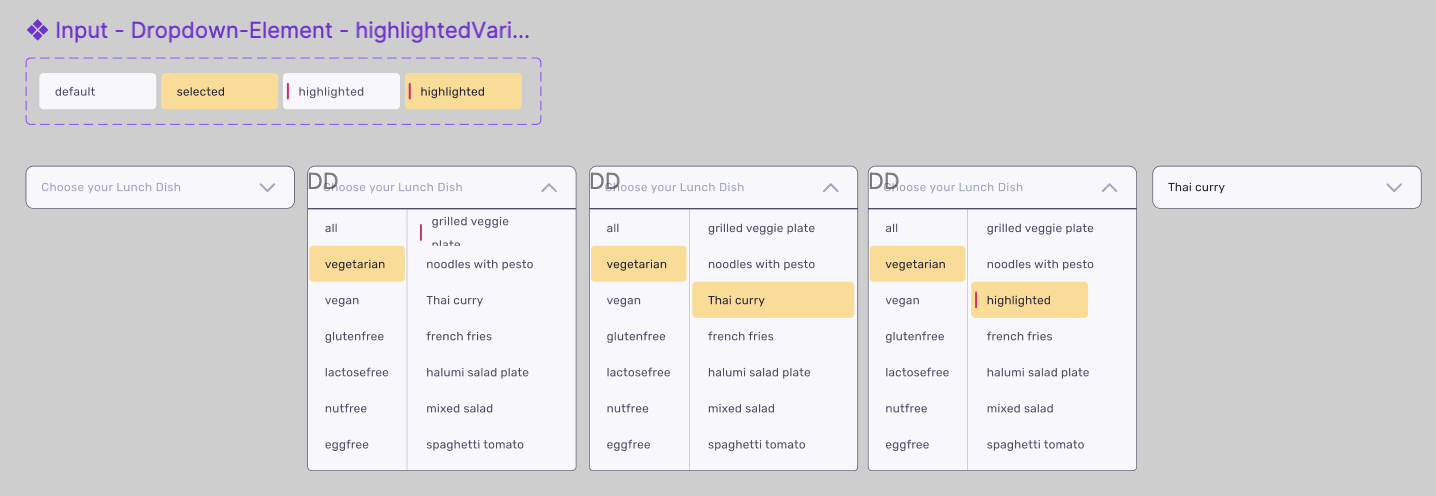
\includegraphics[width=100mm]{figma-prototype-1.png}
    \caption{\centering Figma Prototyp – Dropdown Komponente 1}
    \label{img:figmaPrototype1}
\end{figure}

\begin{figure}[!htb]
    \centering
    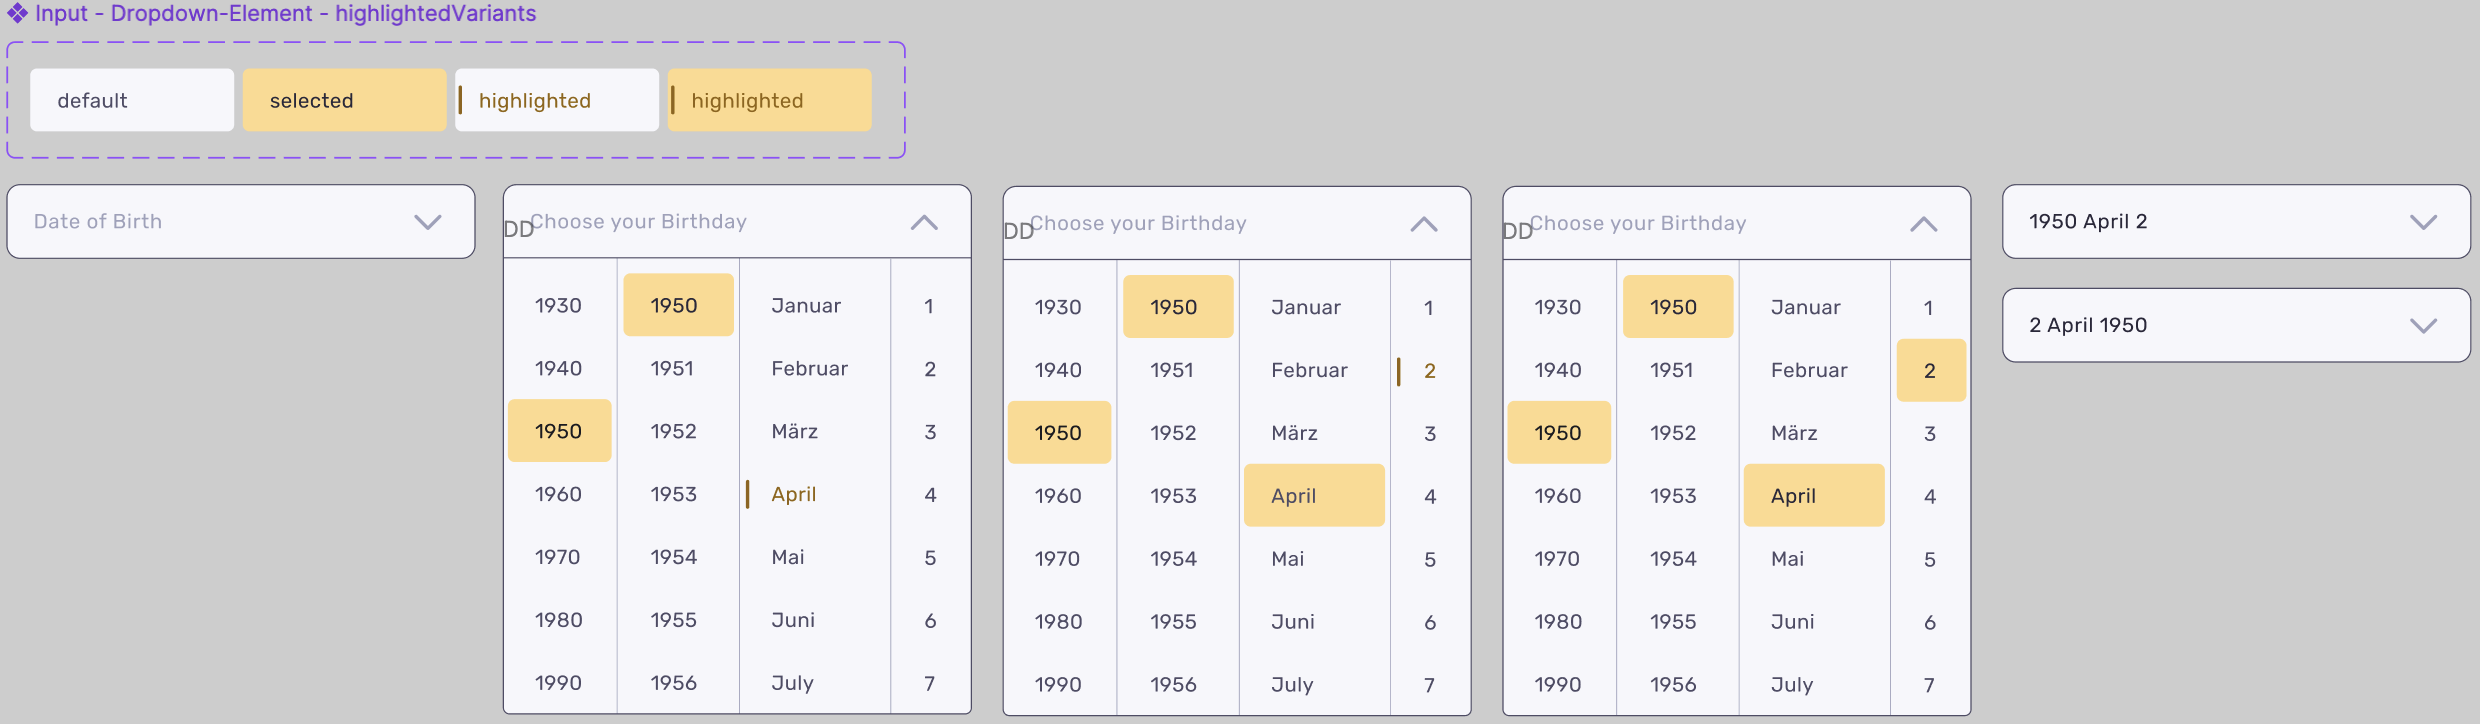
\includegraphics[width=100mm]{figma-prototype-2.png}
    \caption{\centering Figma Prototyp – Dropdown Komponente 2}
    \label{img:figmaPrototype2}
\end{figure}

\begin{figure}[!htb]
    \centering
    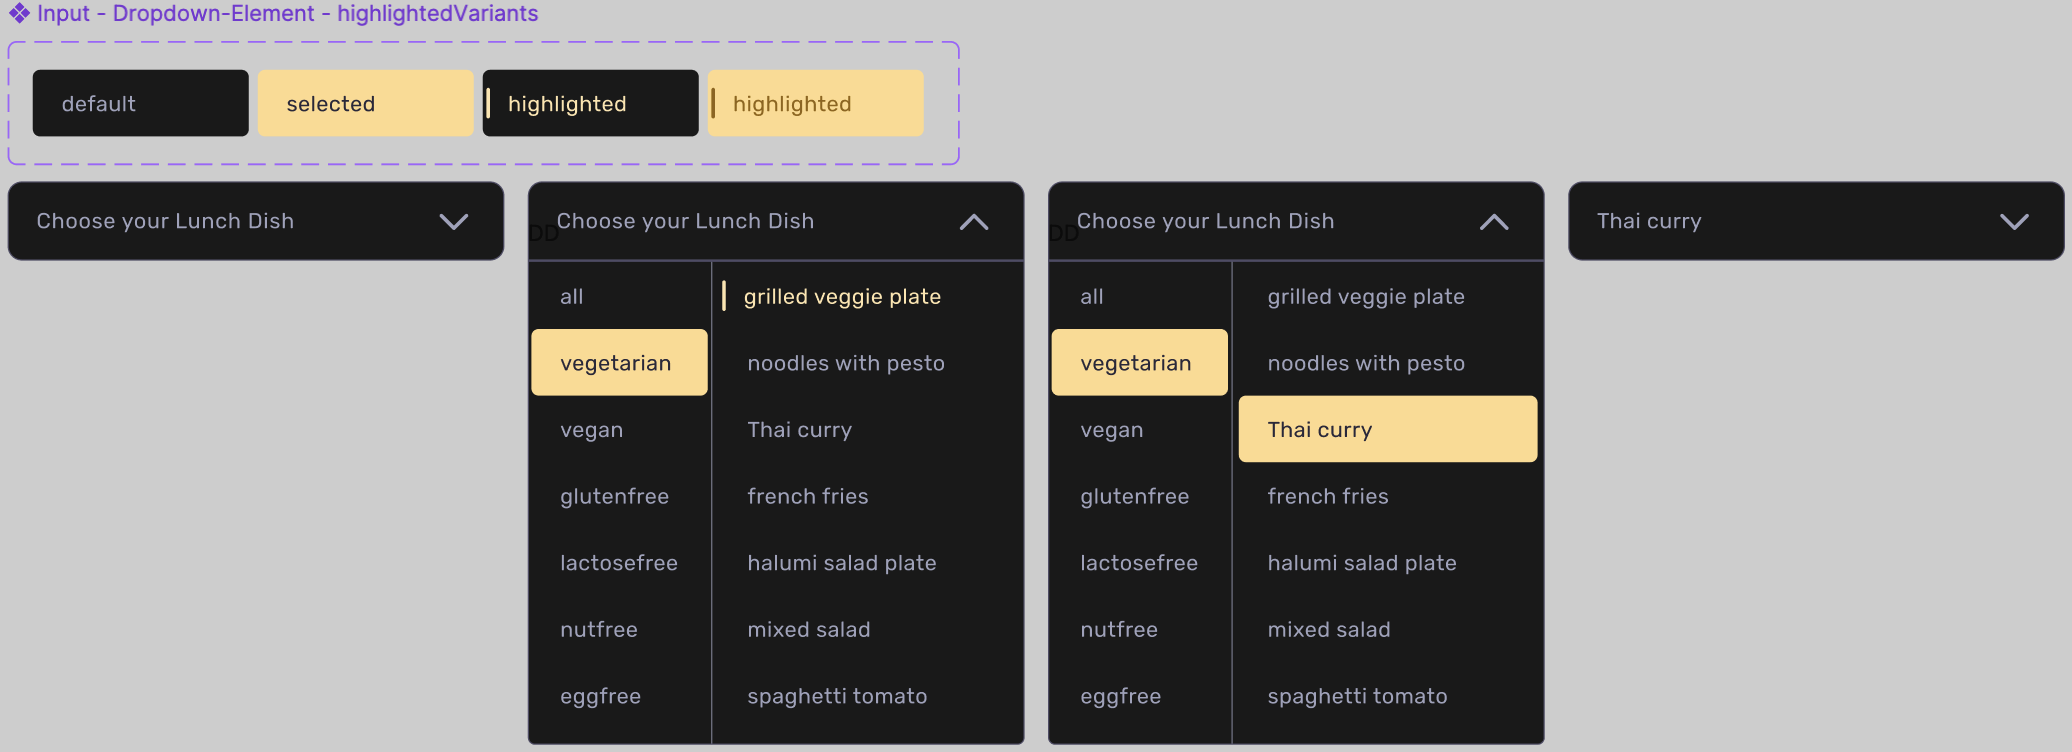
\includegraphics[width=100mm]{figma-prototype-3.png}
    \caption{\centering Figma Prototyp – Dropdown Komponente 3}
    \label{img:figmaPrototype3}
\end{figure}


\subsection{Farbpalette und Kontrast}
\label{sec:colorContrast}

Das Kolibri-Designsystem bietet eine Vielzahl von Farben. 
Der Figma-Prototyp enthält spezifische Anpassungen, so dass die Dropdown-Komponente gut lesbar ist. 
Für den Erhalt einer besseren Nutzerfreundlichkeit gestaltet sich die Farbauswahl aus Abbildung \ref{img:designColors}. 
Diese bietet hohen Kontrast und verbessert somit die Barrierefreiheit der Anwendung. 

\begin{figure}[!htb]
    \centering
    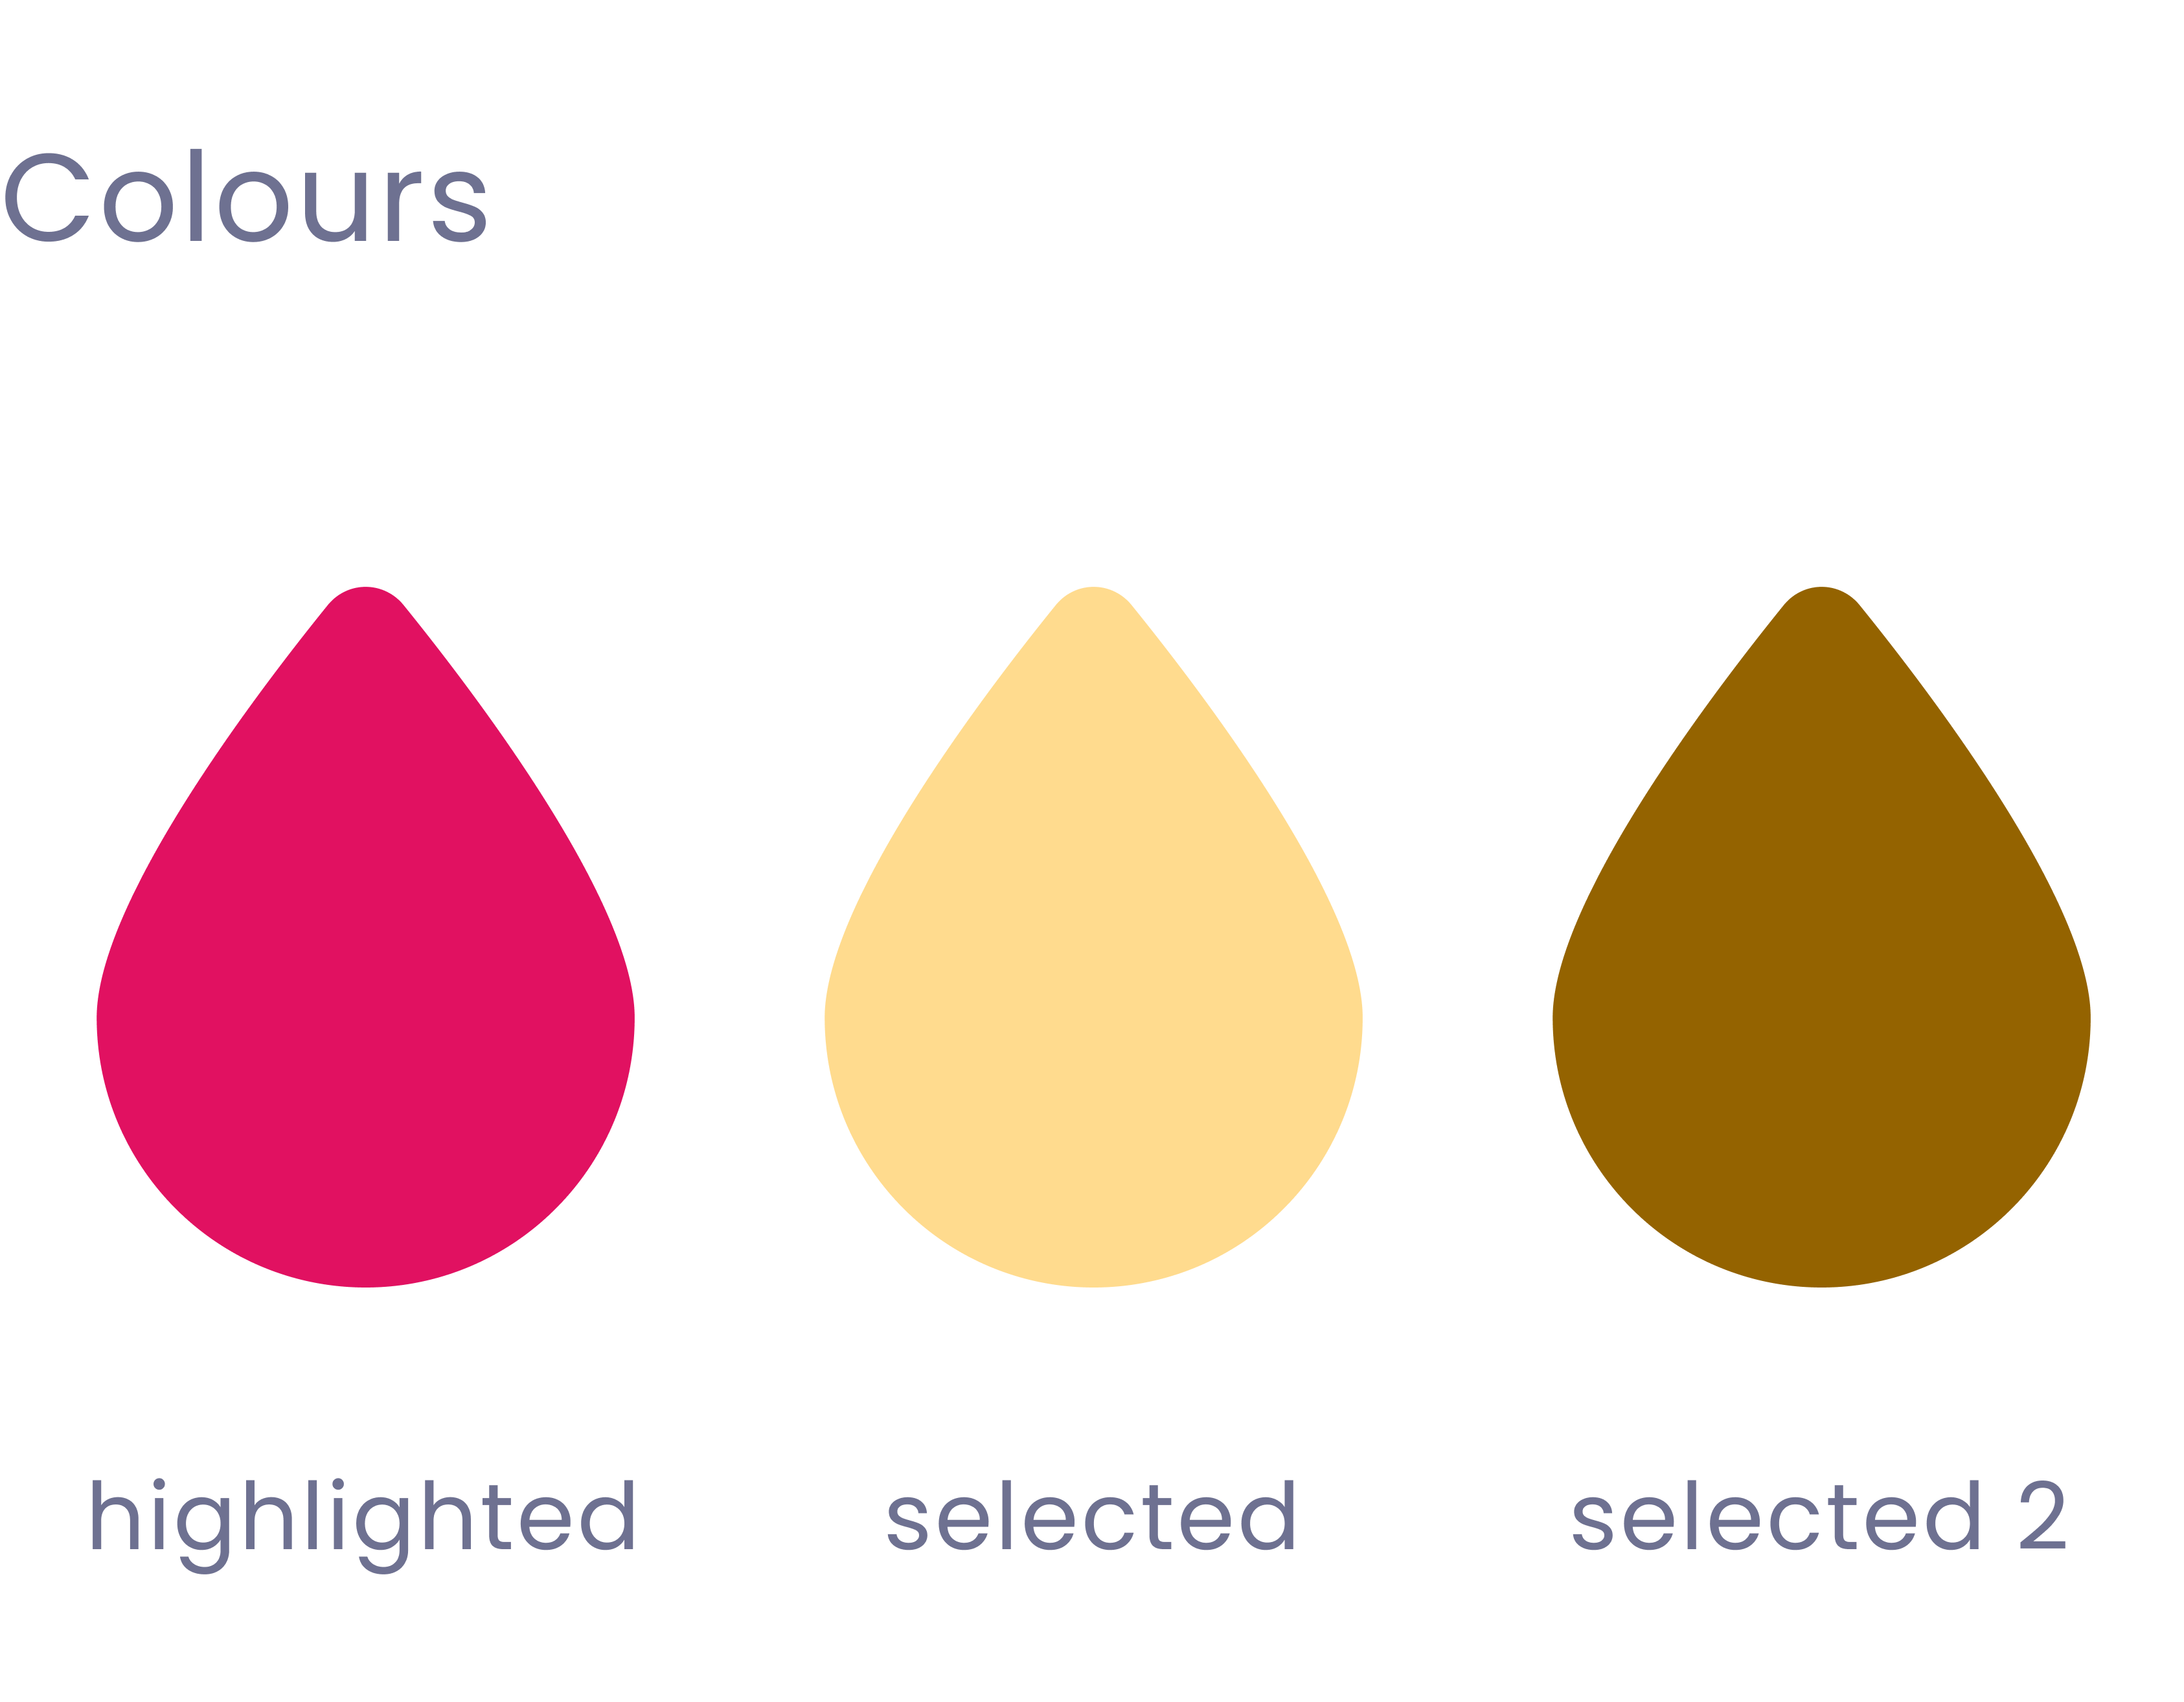
\includegraphics[width=70mm]{design-colors.png}
    \caption{\centering Kolibri Design System – Farbpalette}
    \label{img:designColors}
\end{figure}

\noindent
Die Kolibri-Base Farben erhalten im neuen Dropdown eine angepasste Verwendung:

\begin{itemize}
    \item \textbf{Original} $\rightarrow$ \textbf{Neu}
    \item Kolibri-Light/Yellow/300 $\rightarrow$ selected
    \item Kolibri-Light/Danger/\codestyle{--kb-danger-accent} $\rightarrow$ highlighted
    \item Kolibri-Light/Warning/\codestyle{--kb-warning-dark} $\rightarrow$ cursor position
\end{itemize}

\noindent
Der Code \ref{code:cssImports} zeigt die importierten CSS-Dateien, die als Grundlage für dieses Styling dienen:

\begin{lstlisting}[style = htmlcssjs, caption = CSS Imports, label = code:cssImports]
@import "../../../css/kolibri-base.css";
@import "../../../css/kolibri-light-colors.css";
\end{lstlisting}


\subsection{Layout und Typografie}
\label{sec:layoutTypo}

Die Umsetzung der Dropdown-Komponente des in Figma entworfenen Designs erhält eigenes CSS. 
Nachfolgender Codeausschnitt \ref{code:popoverStyle} zeigt den relevanten CSS-Code, der bei der Gestaltung des Popover- und Option-Styles zur Verwendung kommt:

% todo reduzieren auf wesentliche stellen \& beschreiben => .options-component[popover] inhalt weg kürzen?
\begin{lstlisting}[style = htmlcssjs, caption = CSS für das Popover-Element, label = code:popoverStyle]
@keyframes open {
    0% {
        transform: scaleY(0);
    }
    100% {
        transform: scaleY(1);
    }
}
@keyframes close {
    0% {
        transform: scaleY(1);
    }
    100% {
        transform: scaleY(0);
    }
}
.options-component[popover] {
    position:         absolute;
    z-index:          20;
    max-height:       240px;
    border-radius:    0 0 4px 4px;
    border: 1px       solid #ccc;
    border-top:       none;
    background:       #fff;
    overflow:         hidden;
    align-items:      stretch;
    flex-wrap:        nowrap;
    padding:          0;
    margin:           0;
    box-shadow:       0px 5px 15px #0002;
    animation:        open 300ms ease-in-out;
    transform-origin: top center;
}
.options-component[popover]:popover-open {
    display: flex;
    height:  fit-content;
} 
\end{lstlisting}

Diese CSS-Regeln definieren die Animationen für das Öffnen und Schliessen des Popovers und das grundlegende Styling des Popover-Containers. 
Die \codestyle{@keyframes} regeln die Transformation, während \codestyle{.options-component[popover]} das Layout und das Erscheinungsbild des Popovers steuert. 


\subsection{Implementation der Zustände}
\label{sec:implementStates}

Die Dropdown-Komponente ist so gestaltet, dass sie sowohl für Maus- als auch Tastaturbenutzer optimal funktioniert. 
Das Design der Interaktionen bietet eine intuitive und leicht zugängliche Bedienung der Komponente. 
Spezifische CSS-Klassen erleichtern die Benutzerführung. 
Sie definieren die Styles der hervorgehobenen (highlighted) bzw. ausgewählten (selected) Optionen. 
Der CSS-Code \ref{code:styledElement} zeigt einen Style-Ausschnitt auf ein aktuelles\footnote{
    Element, welches sich unter der Cursor Position befindet
} und selektiertes Element. 

\begin{lstlisting}[style = htmlcssjs, caption = Aktuelle (\codestyle{cursor-position}) und ausgewählte (\codestyle{selected}) Option, label = code:styledElement]
.cursor-position {
    color: var(--kb-hsla-warning-dark);

    &:not(.disabled)::before {
        content:       '';
        position:      absolute;
        left:          7px;
        top:           0.5em;
        bottom:        0.4em;
        transform:     translateX(-50%);

        background:    var(--kb-hsla-warning-dark);
        border-radius: 1px;
        width:         2px;
    }
}
.selected {
    background:    var(--kolibri-color-select);
    border-radius: 4px;
}
\end{lstlisting}

\codestyle{.cursor-position}: Definiert die Hervorhebung der Option, die gerade durch den Cursor\footnote{
    Tastatur-Position-Anker (nicht Maus-Cursor)
} fokussiert ist. 

Eine dunkle Farbe und eine linksseitige Markierung betonen das Element. 
\codestyle{.selected}: Stellt die ausgewählte Option durch einen speziellen Hintergrund und abgerundete Ecken dar. 

Im \codestyle{columnOptionsProjector.js} gibt es Event-Handler, die das Setzen und Entfernen der Highlighting-Klassen steuern:

\begin{lstlisting}[style = htmlcssjs, caption = Steuerung der Highlighting-Klassen, label = code:highlightChange]
const selectOptionItem = (root) => (newOption, oldOption) => {
    const oldItem = getHtmlElementByOption(oldOption, root);
    if (oldItem) {
        oldItem.classList.remove("selected");
    }

    const newItem = getHtmlElementByOption(newOption, root);
    if (newItem) {
        newItem.classList.add("selected");
    }
}; 
const cursorPositionItem = (root) => (newOption, oldOption) => {
    // same structure as selectOptionItem for the cursor-position class
}; 
\end{lstlisting}

\codestyle{selectOptionItem}: Verschiebt die Klasse \codestyle{.selected} und somit die Hervorhebung auf das neue Element. 
\codestyle{cursorPositionItem}: Entfernt bzw. setzt die Klasse \codestyle{.cursor-position} – ähnlich wie beim \codestyle{selectOptionItem}. 

Im Codeausschnitt \ref{code:eventSelection} aus der Datei \codestyle{selectProjector.js} lässt sich das Highlighting durch die Verknüpfung der Optionen und ihrer Events mit den entsprechenden CSS-Klassen steuern. 

\begin{lstlisting}[style = htmlcssjs, caption = Event-Handling für die Auswahl einer Option, label = code:eventSelection]
const projectSelectedValueOptionView = (selectController, popoverElement) => {
    const rootElement = document.createElement("div");
    rootElement.id    = selectController.getId() + "-selected-option";
    rootElement.classList.add("selected-option-component");
    rootElement.setAttribute("data-id", selectController.getId());
    
    const selectedOptionContainer     = document.createElement("div");
    selectedOptionContainer.innerHTML = selectController.getSelectedValueOption().getLabel();
    selectedOptionContainer.onclick   = togglePopover;
    selectedOptionContainer.classList.add("selected-value");
    
    rootElement.append(selectedOptionContainer);
    return [rootElement, selectedOptionContainer];
}; 
\end{lstlisting}

\codestyle{projectSelectedValueOptionView}: Erstellt die Ansicht für die ausgewählte Option und verknüpft die Klick-Events mit dem Umschalten des Popovers. 
Diese Kombination von CSS und JavaScript bietet dem Highlighting und der Auswahl von Optionen in der Dropdown-Komponente eine effektive und visuell ansprechende Umsetzung. 


\subsection{Optionen und Scrollbar-Styling}
\label{sec:sizeLayoutChanges}

Diese CSS-Regeln gestalten die Optionen einer einzelnen Spalte sowie das Scroll-Verhalten des Containers. 
Das \codestyle{.options-column} aus Code \ref{code:optionStyling} definiert das Layout sowie weitere Listen-abhängige Eigenschaften, während das \codestyle{.option-item} das Erscheinungsbild und die Interaktivität der einzelnen Optionen festlegt. 

\begin{lstlisting}[style = htmlcssjs, caption = Optionen und Scrollbar-Styling, label = code:optionStyling]
.options-column {
    position:    relative;
    width:       100%;
    overflow-y:  scroll;
    overflow-x:  hidden;
    max-height:  240px;
    min-height:  100%;
    padding:     5px;
    flex-grow:   2;
    flex-shrink: 1;
}
.option-item {
    position:      relative;
    padding:       10px 20px;
    display:       block;
    cursor:        pointer;
    width:         100%;
    line-height:   1.2;
    overflow:      hidden;
    text-overflow: ellipsis;
} 
\end{lstlisting}

Die Nutzung von den CSS-Styles im JavaScript stellt sicher, dass die dynamischen Klassen und Stile bei den Elementen bei Erstellung oder Aktualisierung ihre Anwendung finden. 
Das Beispiel \ref{code:cssSyleInJs} aus den Dateien \codestyle{selectProjector.js} und \codestyle{columnOptionsProjector.js} verwenden die erwänhten CSS-Klassen:

\begin{lstlisting}[style = htmlcssjs, caption = CSS-Styles im JavaScript, label = code:cssSyleInJs]
// selectProjector.js
const projectOptionsView = (selectController) => {
    const optionsContainer = document.createElement("div");
    optionsContainer.id    = selectController.getId() + "-options";
    optionsContainer.classList.add(optionsClassName);
    optionsContainer.setAttribute("popover", "auto");
    // more popover logic
};

// columnOptionsProjector.js
const projectOption = (selectedOptionController, option, optionType, cursorPositionController) => {
    const item     = document.createElement("div");
    item.innerHTML = option.getLabel();
    item.setAttribute("data-id"   , elementId(option));
    item.setAttribute("data-value", option.getValue());
    item.setAttribute("data-label", elementDataLabel(option));
    item.classList.add(optionClassName);
    item.classList.add(optionType + "-" + optionClassName);
    // more option logic
}; 
\end{lstlisting}

Dieser JavaScript Code erstellt die HTML-Elemente und ergänzt die CSS-Klassen, um das Styling und die Funktionalität sicherzustellen. 
Das \codestyle{selectProjector.js} erstellt und stylt den Popover-Container, während das \codestyle{columnOptionsProjector.js} die einzelnen Options-Elemente gestaltet. 
Diese Kombination aus CSS und JS stellt sicher, dass die Dropdown- und Popover-Komponenten korrekt angezeigt und interaktiv sind. 


\subsection{Prototyping und Benutzerfeedback}
\label{sec:userFeedbackPtototyping}

Der Einsatz von interaktiven Figma-Prototypen ist hilfreich beim Evaluieren der initialen Benutzerfreundlichkeit und intuitiven Bedienung. 
Mit der Integration der Rückmeldungen von Benutzerinteraktionen in das Design verbessert sich die Usability kontinuierlich. 
Beispiele für die Prototypen und die verschiedenen Zustände der Dropdown-Komponente sind in der oberen Hälfte des Bildes \ref{img:figmaPrototype1} ersichtlich. 

Die Gestaltung der Auswahlkomponente umfasst sowohl visuelle als auch funktionale Aspekte. 
Gezielte CSS-Anpassungen und ein durchdachtes Interaktionsdesign finden in der Realisierung ihren Platz. 
Das Ziel ist, eine ansprechende und benutzerfreundliche Komponente zu schaffen. 
Sie fügt sich nahtlos in das Kolibri-Designsystem ein und überzeugt gleichzeitig durch optimierte Les- und Bedienbarkeit. 


\section{Interaktionen} % todo controll bullets with table and paragraph after
\label{sec:interaction}

Damit ein gemeinsames Verständis entsteht, gilt es für die Bedienung der Komponente Regeln festzulegen. 
Wie in den Grundlagen bereits beschrieben kann sich ein Wert aus dem Optionen-Container in verschiedenen Zuständen befinden. 
In diesem Absatz spielen Selektion, Highlight und Cursor Position eine Rolle. 
Zur Auffrischung: 

\begin{itemize}
    \item \textbf{\emph{Selektion}}: Ausgewählter Wert der Spalte
    \item \textbf{\emph{Highlight}}: Element unterhalb des Mauszeigers
    \item \textbf{\emph{Cursor Position}}: Position (Element) der Tastatur
\end{itemize}

\noindent
Bei der Festlegung der Maus-Interaktion fällt die Entscheidung auf folgendes:

\begin{itemize}
    \item \textbf{mouseover}: visuelles Highlighting des Elements ohne Selektionsänderung
    \item \textbf{click}: Änderung der Cursor Position \& Selektionsänderung
\end{itemize}

\noindent
Die Tastatur-Steuerung mit den Pfeiltasten hingegen hält sich an diese Bedienungen:

\begin{itemize}
    \item Änderung der Cursor Position
    \item keine Selektionsänderung
\end{itemize}

\noindent
Als Basis für den ersten Projektor der neuen Komponente ergeben sich aus den oben genannten Regeln folgende Interaktionen (Tabelle \ref{table:interactionNewComponent}). 

\import{../tables}{d.newComponent.tex}

Das Undo und das Redo auf der Komponente erhält im ersten Projektor keine spezielle Definition. 
Gewisse Verhaltensweisen finden sich im geschlossenen als auch offenen Zustand der Komponente wieder. 
Anders als bei den existierenden Komponenten, ist bei der Neuen die Leertaste neu belegt. 
Ist die Liste bereits offen, selektiert diese Interaktion den sich aktuell unter der Cursor Position befindliche Wert. 
Andere Projektoren können eigene Interaktionen definieren. 


\section{Prinzipien \& Regeln}
\label{sec:principleRules}

Diverse Prinzipien garantieren einen stabilen und verständlichen Code. 
Ein Ansatz ist, alle Objekte so immutable als möglich zu halten. 
Dadurch lassen sich unerwartete Änderungen verhindern. 
Weiter gilt es, die Bestandteile im KISS-Stil umzusetzen. 
Dazu zählt, dass die einzelnen Objekte und Funktionen möglichst privat zu gestalten sind. 
Die Bausteine sind kurz und übersichtlich aufzubauen. 
Zu diesem Zweck soll Separation of Concern zum Einsatz kommen, so dass jede Funktion nur eine Aufgabe zu erfüllen hat. 
Damit der Code einfach und lesbar bleibt bzw. wird, gilt es, Entscheidungen zu treffen. 
Zu diesen Entschlüssen zählt das bewusste Weglassen von Funktionalität und somit auch Komplexität. 

Beim Implementieren ist darauf zu achten, den Code sauber zu formatieren. 
Zudem ist es sinnvoll, die Änderungen regelmässig mit dem Code-Analyse-Tool von Intellij auf ihre Qualität zu prüfen. 
Diese Prinzipien und Regeln unterstützen eine ordentliche Entwicklungsumgebung für eine stabile Komponente. 
Das Kapitel Patterns bietet eine weitere Möglichkeit den Code strukturiert zu halten. 


\section{Patterns}
\label{sec:patterns}

In diesem Projekt finden sich einige Code-Patterns wieder. 
Die Wichtigesten wie Null-Object, Projector und Decorator sind in den nachfolgenden Unterkapitel genauer erläutert. 
Eine weitere Rolle spielt unter anderem die Master-Detail-View, aber im Zusammenhang mit der Komponente eher nebensächlich. 
Zudem ist die Anwendung nicht typisch bzw. genau abgegrenzt. 
Die Implementation erhält durch die verwendeten Patterns eine Struktur und läuft stabiler. 


\subsection{Null Object Pattern}
\label{sec:nullPattern}

Ein Pattern, welches im Verlauf der Arbeit eine wichtige Rolle eingenommen hat, ist das Null-Object Pattern\citemarktext{
    [\cite{nullObjectPattern}]
}. 
Null hat den Nachteil, dass alle Funktionsaufrufe darauf zu Fehlern führen. 
Das Null-Object besteht aus vordefinierten Default-Werten und besitzt für alle Funktionen eine \emph{Do-Nothing}-Implementation. 
Durch die Verwendung dieses speziellen Objekts entfällt eine ansonsten notwendige Nullwertprüfung. 
Zudem ist jedes erstellte Null-Object wertegleich. 

Eine Null-Option ist notwendig, um eine Selektion zurücksetzen zu können. 
Die Verwendung des Null-Objects findet sich an mehreren Stellen des Codes wieder. 
Die Definition der angewendeten Null-Option zeigt der nachfolgende Code. 

\begin{lstlisting}[style = htmlcssjs, caption = Null-Option Definition, label = code:nullOption]
/** @private @returns { OptionType } */
const reset = () => {
    return Option(null, null);
};

/** @public @type { OptionType } */
const nullOption = reset();
\end{lstlisting}

Mit dem Erhalt des Typs \codestyle{Option} bietet die Konstante die selbe Funktionalität wie die gewünschten Objekte. 
Der Codeausschnitt \ref{code:nullOption} befindet sich in der Datei \codestyle{optionsModel.js}. 
Mehr zur File Aufteilung ist in den nächsten zwei Unterkapiteln zu lesen. 


\subsection{Projector Pattern}
\label{sec:projectorPattern}

Das Projector Pattern\citemarktext{
    [\cite{projectorPattern}]
} basiert auf dem verbreiteten Model-View-Controll Pattern. 
Das Model verwaltet die dargestellten Daten. 
Zudem enthält die Komponente des Patterns die Geschäftslogik und verarbeitet die Regeln und Anfragen für die Daten. 
Ein Controller generiert privat gehaltene Modelle. 
Dabei stellt dieser nur die notwendigen Funktionen zur Verfügung. 
Diese Funktionen können Getter, Setter und Listener der observierten Modelle und Werte sein. 
Der Projektor bindet Daten-Modelle über den Controller an die View. 
Auf der anderen Seite bindet sich die View an die Models. 
Aus den Bindings und den Daten generiert ein Projetor die passende View. 
Die View ist passiv und hat keine Kenntnis über die anderen Komponenten. 

Dieses Pattern zeigte sich als eines der Wichtigsten für die Erstellung der neuen Komponente. 
In den folgenden Grafiken sind Models als Zylinder, Controller als schiefes Rechteck und Projectors als Oval dargestellt. 
Die Raute mit Option ist ein Daten-Typ, der über das gesamte Projekt seine Anwendung findet. 
Das \codestyle{starter.js} beinhaltet alle Bestandteile, welche für eine Anwendung notwendig sind. 
Eine genauere Beschreibung des Puzzles folgt im Unterkapitel \textbf{\nameref{sec:decoratorPattern}}. 
Die erste Implementation, welche dieses Pattern verwendet, ist auf Abbildung \ref{img:diagramSelectComponentOld}. 

\begin{figure}[!htb]
    \centering
    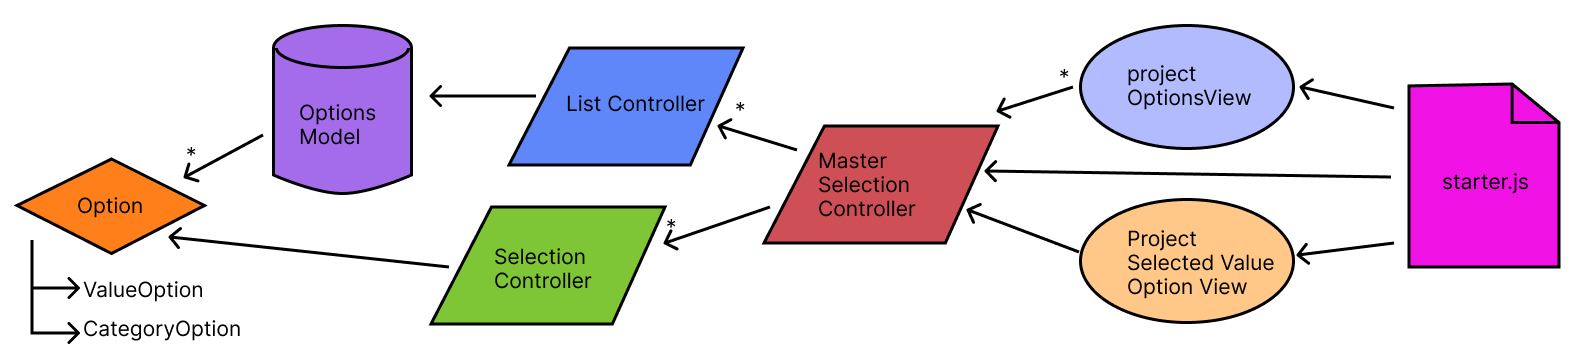
\includegraphics[width=120mm]{diagram-select-component-old.png}
    \caption{\centering Diagramm Select Component – erste Version}
    \label{img:diagramSelectComponentOld}
\end{figure}

Diese Version zeigt noch viel Komplexität und duplizierenden Code in den einzelnen Funktionen. 
Eine genaue Analyse der Komponente zeigt, dass sich das Pattern zwei Mal anwenden lässt. 
Die neue Aufteilung ergibt die zwei folgenden Abbildungen \ref{img:diagramColumnComponent} und \ref{img:diagramSelectComponent}. 
Die Implementation der dargestellten Diagramme resultiert aus einem Refactoring im grösseren Rahmen. 

\begin{figure}[!htb]
    \centering
    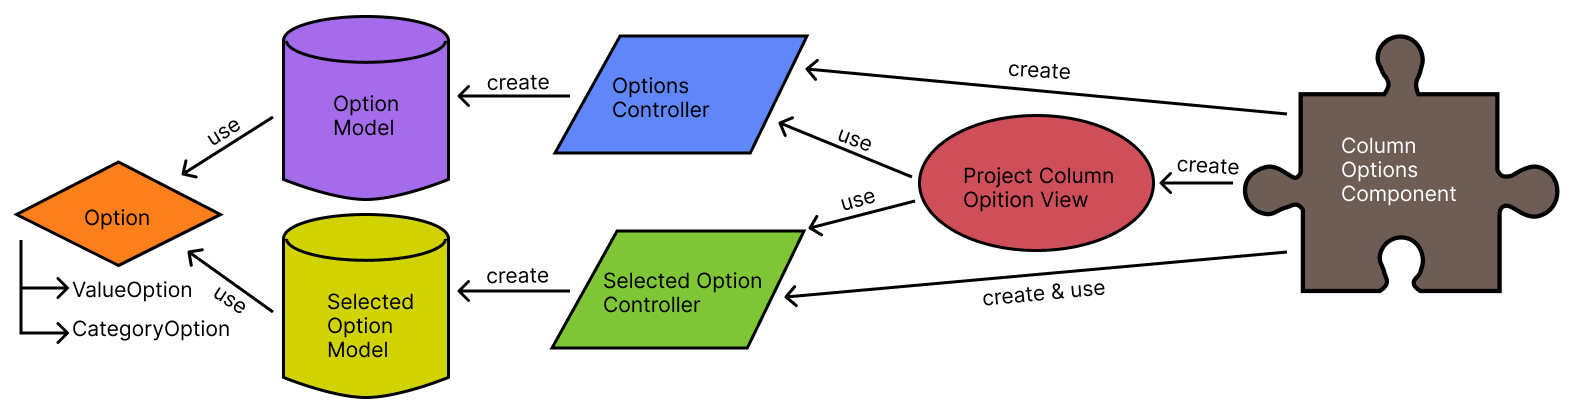
\includegraphics[width=120mm]{diagram-column-component-with-desc.png}
    \caption{\centering Diagramm \codestyle{ColumnComponent}}
    \label{img:diagramColumnComponent}
\end{figure}

Zum einen findet sich das Projector Pattern in einer einzelnen Spalte in der Options-Liste wieder. 
Pro Kolonne existiert eine Auswahl und eine Menge von Optionen. 
Diese beiden Bestandteile besitzen je ein eigenes Model und einen eigenen Controller. 
Der Projektor generiert eine gemeinsame View und bindet diese an die beiden Controller. 
Bei einer Anwendung übernimmt die \codestyle{ColumnComponent} die Verwaltung gewisser Bausteine (Mehr dazu später). 

\begin{figure}[!htb]
    \centering
    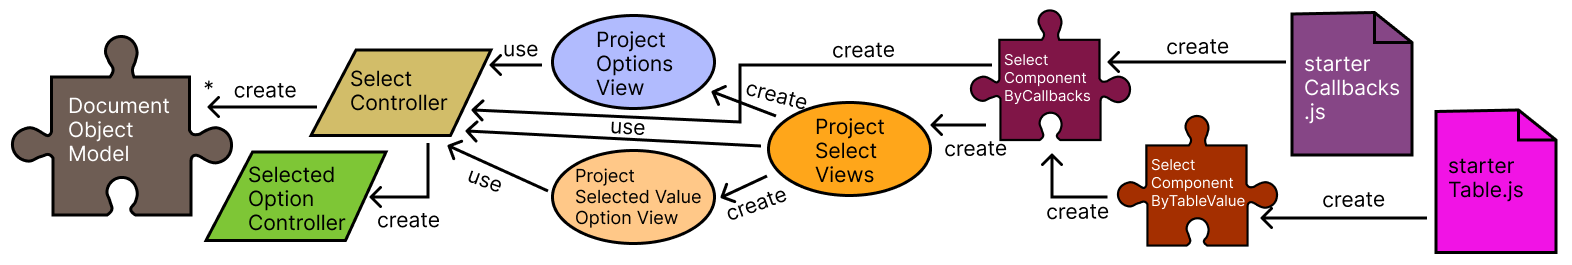
\includegraphics[width=120mm]{diagram-select-component-with-desc.png}
    \caption{\centering Diagramm \codestyle{SelectComponent}}
    \label{img:diagramSelectComponent}
\end{figure}

Die Anwendungskomponente einer Column findet sich als Bestandteil des zweiten Projector Pattern wieder. 
Ein \codestyle{SelectController} verwaltet eine bis mehrere \codestyle{ColumnComponent}s als auch ein Element für die Tastaturnavigation. 
Die sogenannte Cursor Position verwendet im Hintergrund ebenfalls einen \codestyle{SelectedOptionController}. 
Dieser ist derselbe wie in der Abbildung \ref{img:diagramColumnComponent} und findet hier eine Wiederverwendung. 
Für die Definition der Bindings greifen die einzelnen Projektoren auf den selben Controller zu. 
Der Master-Detail-Aufbau der neuen Komponente findet sich in der Aufteilung der Projektoren wieder. 
Der Detail-Baustein kümmert sich um die aktuelle Auswahl und das Eingabefeld. 
Die Master-Komponente verwaltet alle Spalten mit den Kategorie- und Werte-Optionen, sowie dessen Bindings. 
Eine weitere Funktion ist die Einbettung der beiden Projektoren in eine gemeinsame View. 
Auch diese Projector Pattern Anwendung schliesst mit einer Component – der \codestyle{SelectComponent} – ab. 
Mehr zu dieser und der \codestyle{ColumnComponent} steht im nächsten Kapitel. 


\subsection{Decorator Pattern}
\label{sec:decoratorPattern}

Ein Decorator\citemarktext{
    [\cite{decoratorPattern}]
} bietet zusätzliches Verhalten ohne das Originale Objekt zu verändern. 
Dabei lassem sich verschiedene Funktionen kombinieren. 
Dieses Pattern ermöglicht die Erstellung eines modularen und anpassbaren Codes. 
In diesem Projekt unterstützt es die Gestaltung und Erweiterung der Auswahlkomponente. 

Wie im vorherigen Kapitel erwähnt, besteht die neue Komponente unter anderem aus zwei sogenannten Component-Bausteinen. 
Die Decorator sind in den Abbildungen \ref{img:diagramColumnComponent} und \ref{img:diagramSelectComponent} als Puzzle dargestellt. 
Diese Bestandteile kombinieren die Funktionalität des Controllers mit der Erstellung der View. 
Dadurch lässt sich die neue Komponente einfacher anwenden. 

\begin{lstlisting}[style = htmlcssjs, caption = \codestyle{SelectComponentByTableValue} dekoriert \codestyle{SelectComponentByCallback}, label = code:componentDecorator]
const SelectComponentByTableValues = (
    selectAttributes,
    optionsTable,
    sortColumnOptionsAlphabetical = false
) => {
    /* code for mapping between table and callbacks */
    const component = SelectComponentByCallbacks(selectAttributes, callbacks);
    return {
        ...component,
    };
};
\end{lstlisting}

Ein weiterer Einsatzort ist in der Abbildung \ref{img:diagramSelectComponent} aus dem Vorkapitel zu sehen. 
Der \codestyle{SelectComponentByTableValue} in Code \ref{code:componentDecorator} dekoriert die \codestyle{SelectComponentByCallback}. 
Damit bietet die neue Komponente zwei verschiedene Möglichkeiten der Anwendung. 
Das nächste Kapitel geht genauer auf den Master-View-Bereich des \codestyle{SelectProjector}s – Abbildung \ref{img:diagramSelectComponent} – ein. 


\section{Dropdown-Container}
\label{sec:dropdownContainer}

Für die Darstellung aller Optionen (zu gegebener Zeit) stehen verschiedene Varianten zur Auswahl. 
Eine Möglichkeit ist, den Container als HTML-Dialog zu gestalten. 
Die vorhandenen Funktionen sind jedoch nicht für diese Komponente geeignet. 
Für den gewünschten Zweck erfordert das Dialog-Element noch einiges an benutzerdefinierter Anpassung. 

Eine weitere Variante ist, ein normales \codestyle{div} als Options-Container zu verwenden. 
Dies erfordert ebenfalls einen enormen Implementationsaufwand. 
Eine Andwendung dieses Ansatzes findet sich in der ersten Version der Komponente. 
Hierbei eröffnet sich das Problem von der Inkonsistenz zwischen UI und Controller. 
Zudem ist es möglich, dass unerwünscht mehrere Dropdown-Container gleichzeitig offen sind. 

Als dritte Möglichkeit bietet sich die Popover-API an. 
Seit 2024 unterstützen alle gängigen Browser diese Schnittstelle. 
Durch das Refactoring der Variante mit dem normalen Div-Container resultiert eine Version mit der Anwendung dieser API. 
Im Gegensatz zu den beiden oben erwähnten Container-Implementationen reduziert sich durch diese Schnittstelle der Zusatzaufwand. 
Der Grundaufbau des Popover-Container ist im folgenden Code \ref{code:popoverExample} dargestellt. 

\begin{lstlisting}[style = htmlcssjs, caption = Popover-Container Beispiel, label = code:popoverExample]
<div popover="auto"
     id="select-component-0-options" 
     class="options-component" 
> <!-- content --> </div>
\end{lstlisting}

Bei diesem Codeausschnitt ist wichtig, dass das Attribut \codestyle{popover} den Wert \codestyle{auto} erhält. 
Dies bewirkt, dass die Popover sich automatisch schliessen, wenn ein Klick ausserhalb des Container passiert. 
Das Öffnen und Schliessen des Dropdown-Elements lässt sich über das \codestyle{popovertarget}-Attribut auf der Bedienkomponente steuern. 
Dieses Target enthält die \codestyle{id} des Div-Containers mit dem Attribut \codestyle{popover}. 
Als Alternative dazu besteht die Möglichkeit, das Popover über JavaScript zu steuern. 
Hierbei besteht die Möglichkeit auf den Status und das Event des Togglens zuzugreifen. 
Diese Funktionalitäten erlauben den Controller konsistent zum UI zu halten. 


\section{Performance}
\label{sec:performance}

Mit der Kenntnis des Rendering Prozesses einer Webseite lässt sich eine gute Performance umsetzen. 
Dieser Ablauf ist im Kapitel \textbf{\nameref{chap:background}} unter \textbf{\nameref{sec:structureRendering}} genau beschrieben. 
Die folgende Abbildung \ref{img:renderingProcessRecap} zeigt die Kernelemente des Prozesses nochmals im Überblick. 

\begin{figure}[!htb]
    \centering
    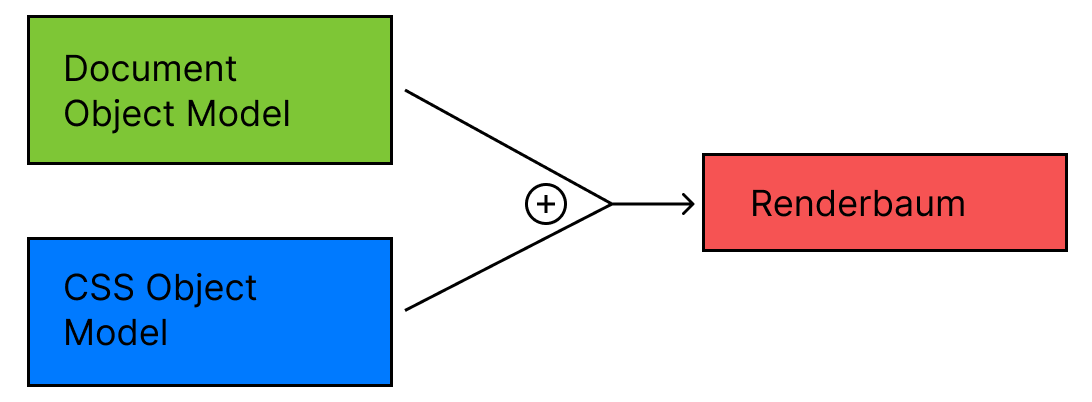
\includegraphics[width=80mm]{rendering-process.png}
    \caption{\centering Rendering Prozess}
    \label{img:renderingProcessRecap}
\end{figure}

Zur Auffrischung die wichtigesten Punkte nochmals: 
Der Browser kann die Webseite maximal 60 Mal pro Sekunde neu zeichnen. 
Änderungen am DOM (Abbildung \ref{img:renderingProcessRecap}) lösen das Rendern aus. 

Deswegen müssen viele kleine Änderungen ausserhalb des Browser-DOMs\footnote{
    Im Renderbaum verwendeter und im Browser angezeigter DOM
} – am besten in einem sogenannten Shadow-DOM – geschehen. 
Ein Shadow-DOM ist ein Teilbaum, welcher nicht am Browser-DOM angehängt ist. 
Für einen reibungslosen Ablauf ist es sinnvoll, die Änderungen nach dem Abhängen des Elternknotens zu vollziehen. 
Nach den Änderungen ist der Teilbaum wieder an den gewünschten Ort einzuhängen. 

\begin{lstlisting}[style = htmlcssjs, caption = Performance Optimierung (aus \codestyle{columnOptionsComponent.js}), label = code:performanceOptimization]
const addAllOptions = (options) => {
    const placeHolder = createHolder();
    columnView.replaceWith(placeHolder);
    if (options.length > 50) {
        // same work as else but async
    } else {
        options.forEach((option) => {
            optionsController.addOption(option);
        });
        updateScrollbar(columnView);
        placeHolder.replaceWith(columnView);
    }
};
\end{lstlisting}

Code \ref{code:performanceOptimization} ist eine Stelle, die diese Technik verwendet. 
Das Anzeigen eines Platzhalters mit einem Lade-Indikator an der Ursprungsstelle bewirkt, dass der Nutzer ein Feedback erhält. 
Sobald der SpaltenContainer abgekoppelt ist, lädt die Funktion die Optionen in den Shadow-DOM. 
Nach Abschluss ersetzt sich der Lade-Indikator der originalen Stelle im Renderbaum durch den Container mit den neuen Elementen. 

Weiter ist darauf achten, dass CSS-Klassen\citemarktext{
    [\cite{efficientDomManipulation}]
} an Stelle von Inline-Styles\footnote{
    Offizieller Begriff: Element attached style $\Rightarrow$ Styles direkt im HTML-Element mit Attribut \codestyle{style} definiert
} ihre Verwendung finden. 
Die Selektoren sollten hierarchisch möglichst flach und nicht verschachtelt sein. 
Wenn es die Situation erlaubt, ist es besser, nicht mit \codestyle{innerHTML} zu arbeiten. 
In diesem Projekt ist es für die Anzeige der Label jedoch nötig \codestyle{innerHTML} zu nutzen. 
Dies liegt daran, dass ein Label auch ein Bild enthalten kann. 
Generell verwendet die neue Auswahlkomponente keine Inline-Styles. 
Die einzige Ausnahme betrifft das verborgene Eingabefeld. 
Durch den Code \ref{code:inlineStyle} sind die Properties vor dem einfachen Überschreiben\footnote{
    \codestyle{!important} besser nicht verwenden
} geschützt. 

\begin{lstlisting}[style = htmlcssjs, caption = Inline-Style für Input-Feld, label = code:inlineStyle]
inputElement.setAttribute(
    "style", "all:            unset       !important; " +
             "z-index:        -1          !important; " +
             "position:       absolute    !important; " +
             "inset:          5px         !important; " +
             "color:          transparent !important; " +
             "pointer-events: none        !important; "
);
\end{lstlisting}

Die Regeln in Code \ref{code:inlineStyle} sorgen dafür, dass das Input-Feld transparent als auch resetet ist. 
Zudem befindet es sich im Hintergrund und besitzt dieselben Grösse wie der Container mit dem ausgewählten Wert. 


\subsection{Performance Vergleich}
\label{sec:performanceCompare}

Durch die Anpassungen der Performance Optimierung, verschnellert sich die Ladezeit bei grossen Datenmenge enorm. 
Die Testseite enthält vier existierende und vier neue Auswahlkomponenten mit den selben Inhalten wie je eines der Existierenden. 
Je eine der Selects enthält eine grosse Datenmenge von über 4'000 Werten. 
Die folgenden zwei Bilder \ref{img:performanceTestBefore} und \ref{img:performanceTestAfter} zeigen die Messung während des Seitenaufbaus. 

\begin{figure}[!htb]
    \centering
    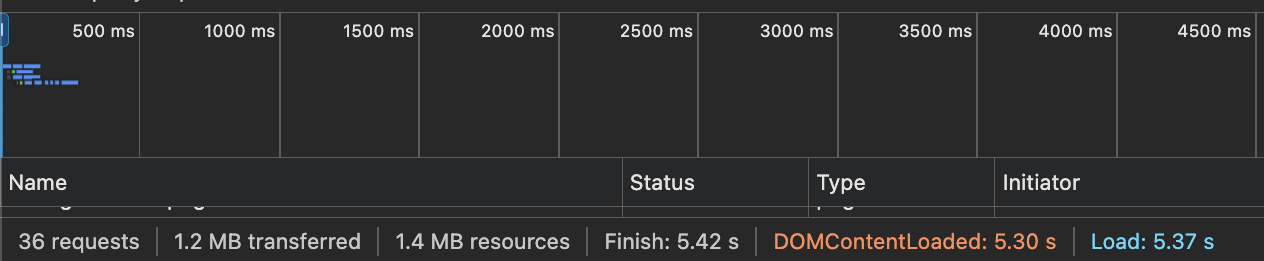
\includegraphics[width=120mm]{performance-before-user-tests-zoom.png}
    \caption{\centering Performance Test vor Anpassungen}
    \label{img:performanceTestBefore}
\end{figure}

Auf der Grafik \ref{img:performanceTestBefore} ist zu sehen, dass der Seitenaufbau der früheren Version mit über 5 Sekunden (rechts unten in blau) sehr lange dauerte. 
Die Implementation führte sehr viele Aktionen auf dem Renderbaum aus. 
Die lange Wahrtezeit bestätigten mehrere Feedbacks der Nutzer, später mehr dazu. 

\begin{figure}[!htb]
    \centering
    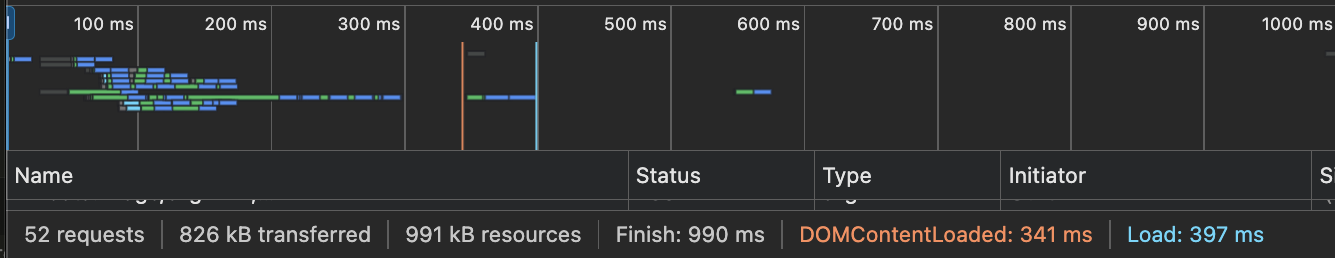
\includegraphics[width=120mm]{performance-after-user-tests-zoom.png}
    \caption{\centering Performance Test nach Anpassungen}
    \label{img:performanceTestAfter}
\end{figure}

Ein Refactoring der früheren Implementation führt zur Auslagerung der aufwendigen Arbeiten auf den Shadow-DOM. 
Dadurch verkürzt sich der Ladevorgang um vier bis fünf Sekunden auf knapp 0.4 Sekunden (rechts unten in blau). 
Der direkte Vergleich zwischen Abbildung \ref{img:performanceTestBefore} und \ref{img:performanceTestAfter} zeigt, dass die Seite um Faktor 13 schneller geladen ist. 
Feedbacks zu den durchgeführten User-Tests mit Programmierern als auch Endnutzern sind im nachfolgenden Kapitel aufgeführt. 


\section{Testing}
\label{sec:testing}

Verschiedene Arten von Tests garantieren die Korrektheit der einzelnen Funktionen und Komponenten. 
Die automatisierten Code-Tests stellen sicher, dass das Aufrufen der gebotenen Funktionalität die gewünschten Änderungen ausführt. 
Komponenten, welche für die Erstellung des UI zusändig sind, prüfen die Existenz von Elementen als auch das Triggern der Events. 
Die User Tests mit unterschiedlichen Personen gewährleisten eine gute Nutzerzufriedenheit als auch die intuitive Anwendung durch Programmierer. 
Die Auswahl der Nutzer fällt auf eine grosse Vielfalt, damit die Resultate unterschiedliche Sichtweisen einbeziehen. 


\subsection{Automatisierte Tests}
\label{sec:automatedTests}

Tests für Komponente der \codestyle{SelectComponent} beweisen die Stabilität des Codes. 
Generell befinden sich die einzelnen Komponenten nach Separation of Concern je in einer eingenen Test-Einheit. 
Dies garantiert das schnelle Auffinden von Bugs und unerwünschtem Verhalten direkt in einer Komponente. 
Auf der Abbildung \ref{img:automatedTests} ist zu sehen, dass eine breite Palette an Kontrollen stattfindet und sauber durchläuft. 

\begin{figure}[!htb]
    \centering
    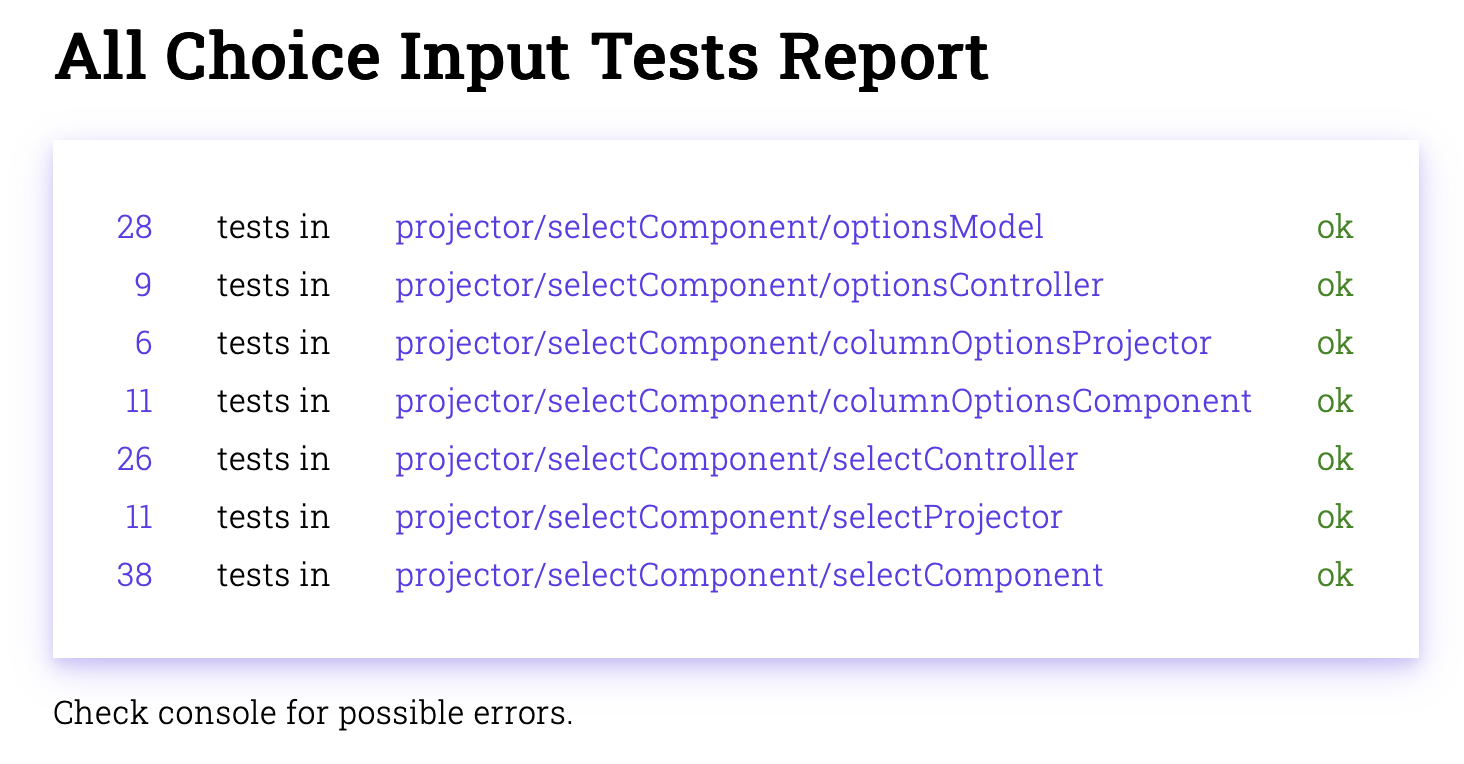
\includegraphics[width=100mm]{automatedTests.png}
    \caption{\centering Automatisierte Tests}
    \label{img:automatedTests}
\end{figure}

Die oberen vier Zeilen auf Abbildung \ref{img:automatedTests} zeigen Tests zu den Bausteinen aus Abbildung \ref{img:diagramColumnComponent}. 
Diese decken den Level der Options bis zur Column ab. 
Die ersten zwei Test-Suites kümmern sich genauer um die Korrektheit der Models und Controller. 
Dabei besteht das erste File aus den Tests der Typen \codestyle{ValueOption} und \codestyle{CategoryOption}. 
Dazu gesellen sich Prüfungen der Komponenten \codestyle{OptionsModel} und \codestyle{SelectedOption\-Model}. 
Der \codestyle{OptionsController} und der \codestyle{SelectedOption\-Controller} finden sich in der Test-Datei wieder. 
Der \codestyle{project\-ColumnOptions\-View}-Test deckt die Kontrolle des Bindings und die Existenz der View-Elemente ab. 
Die Korrektheit des Zusammenspiels zwischen Projektor und Controller findet sich im \codestyle{Column\-Options\-Component}-Testing wieder. 

Die restlichen Test-Bibliotheken decken die Korrektheit der auf Abbildung \ref{img:diagramSelectComponent} sichtbaren Bausteine ab. 
Diese drei Dateien prüfen das Zusammenspiel der Columns als auch der allgemeinen Komponenten-Funktionalitäten. 
In einzelnen Units prüft die \codestyle{SelectController}-Test-Suite verschiedene Varianten der Anwendung. 
In dem \codestyle{projectSelectViews}-Test befindet sich – wie bereits bei der Column – die Prüfungen der Korrektheit der Bindings und View-Elemente. 
Die letzte Datei kümmert sich um die Kontrolle verschieden angewendeter \codestyle{SelectComponent\-ByCallbacks} und \codestyle{SelectComponent\-By\-TableValues}. 
Die breite Abdeckung der Einzelteile garantiert die korrekte Funktion der neuen Komponente. 
Die Tests im nachfolgenden Kapitel sind für eine gute Anwendbarkeit im Code als auch angenehme Benutzung der Auswahlkomponente im Browser notwendig. 


\subsection{Manuelle Tests}
\label{sec:manuelTests}

% 


\subsection{User Tests} % todo
\label{sec:userTests}

% personas im anhang


\subsubsection{Programmierer}
\label{sec:userTestsProgrammer}

% images und text von umfrage im anhang


\subsubsection{Formular-Ausfüller}
\label{sec:userTestsEnduser}

% 


\section{Fazit}
\label{sec:summeryNew}
% todo neu 
Das Kapitel zur neuen Auswahlkomponente umfasst eine umfassende Beschreibung der verschiedenen Aspekte und Überlegungen, die in die Entwicklung eingespielt haben. 
Das Design der Komponente, inspiriert durch das Kolibri-Designsystem, stellt sicher, dass die visuelle Konsistenz und Benutzerfreundlichkeit erhalten bleiben. 
Die spezifischen Designoptionen wie Farbpalette und Layout sind sorgfältig ausgewählt und implementiert, um eine optimale Lesbarkeit und Bedienbarkeit zu gewährleisten. 

Der Einsatz von Figma-Prototypen ist entscheidend, um eine realitätsnahe Vorschau und Benutzerfeedback zu erhalten. 
Dadurch verbessert sich die Benutzerfreundlichkeit kontinuierlich. 
Die Kombination von durchdachten CSS-Anpassungen und einem klaren Interaktionen stellt sicher, dass die Komponente sowohl für Maus- als auch für Tastaturbenutzer zugänglich und intuitiv ist. 

Die Integration von Prinzipien wie KISS und Separation of Concern sowie die Anwendung von Patterns wie Null Object und Projector tragen zur Schaffung eines stabilen und wartbaren Codes bei. 
Der Dropdown-Container ermöglicht eine konsistente und benutzerfreundliche Darstellung der Optionen. 

Die durchgeführten User Tests bestätigten die hohe Usability der Komponente, und die automatisierten Tests gewährleisten eine hohe Codequalität. 
Ein agiles Entwicklungsverfahren ermöglicht durch stetige Optimierung die Entstehung der neuen, effizienten Auswahlkomponente. 
Sie bildet eine solide Grundlage für zukünftige Erweiterungen und Anpassungen. 
